\section{Introduction}

\begin{figure*}[t]
  \centering
  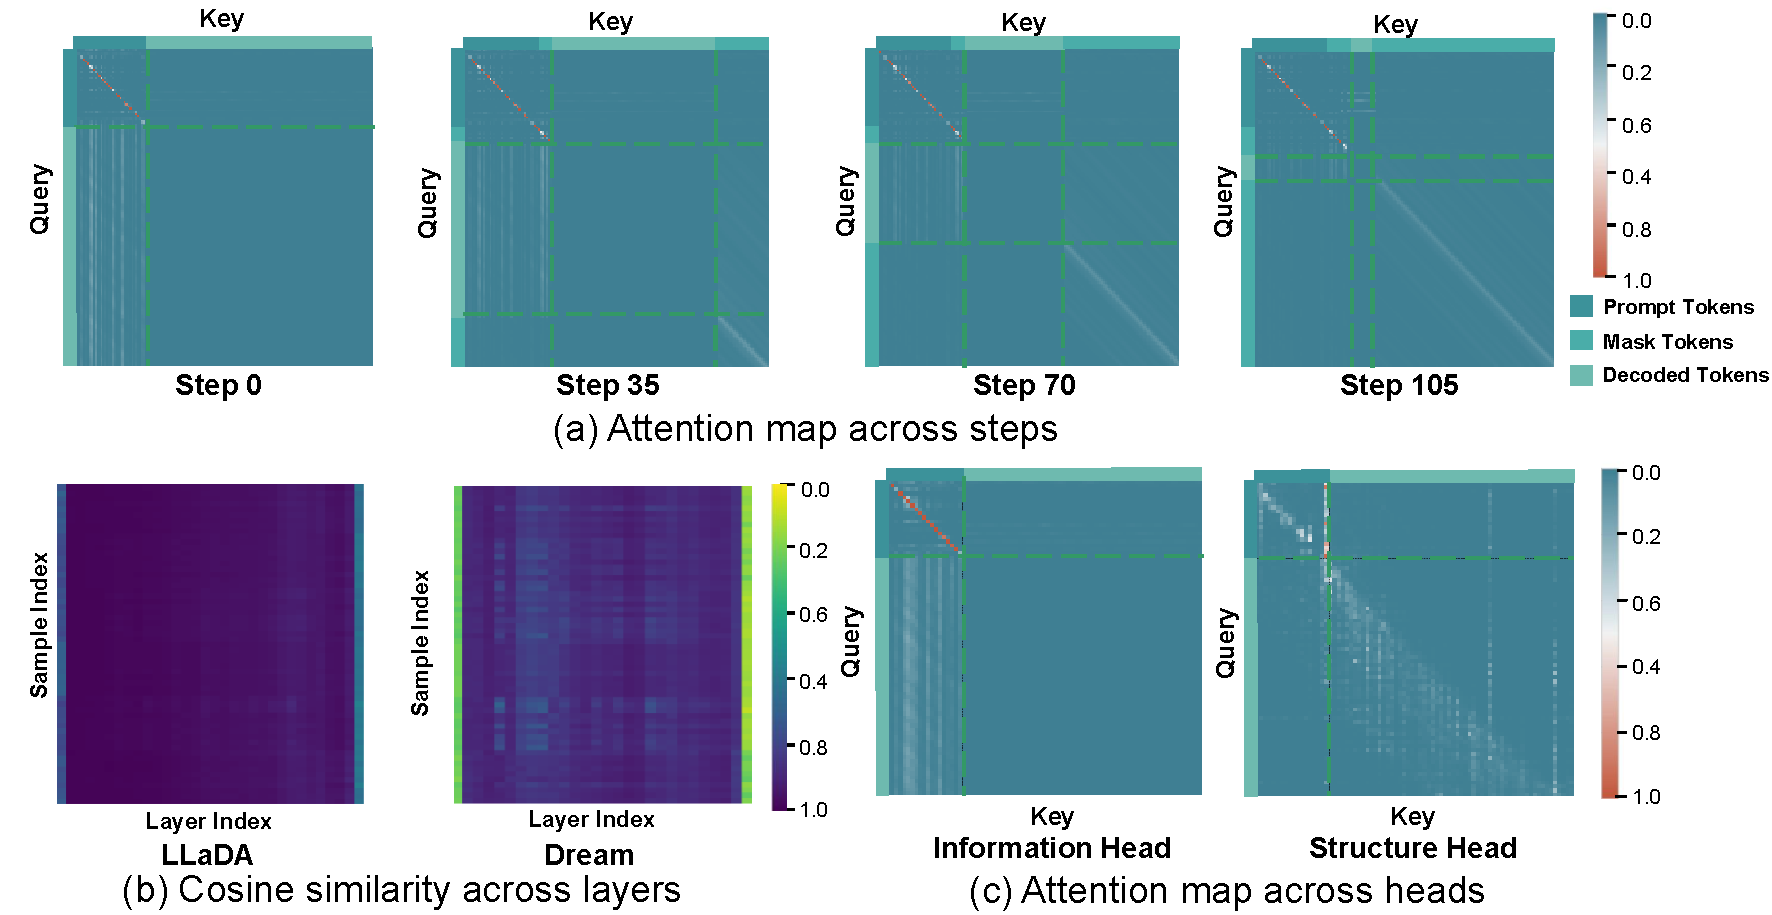
\includegraphics[width=1.0\linewidth]{figure/intro.pdf}
  \caption{
  \textbf{Visualization on attention maps and features in LLaDA.}
    (a) The queries from the mask token tend to clearly concentrate on several ``important'' prompt tokens, indicating they are able to choose the valuable prefix. (b) The first layer and the last layer in diffusion LLMs tend to show significantly lower cosine similarity compared to their adjacent layers, indicating these two layers contribute more than other layers in generation. (c) ``information heads'' tend to focus more on the previous prompts while ``structure heads'' focus more on the mask tokens.
    }
  \label{fig:attention_map}
\end{figure*}

%LLM+ARM+dLLM
Over the past few years, autoregressive language models have dominated text generation~\citep{zhao2023survey}, but their strictly left-to-right decoding enforces sequential inference and limits throughput. Diffusion large language models (dLLMs) lift the latency ceiling by iteratively denoising a fully masked sequence, enabling parallel prediction of all tokens with bidirectional attention for richer contextual reasoning~\citep{genimid,chen2025dpad, wang2025diffusion}. Closed-source systems such as Gemini Diffusion~\citep{genimid} and Mercury~\citep{khanna2025mercury} have already pushed this paradigm to production scale, sustaining thousand-token-per-second decoding and proving its commercial viability. Open-source counterparts, LLaDA-8B (trained from scratch)~\citep{nie2025large} and Dream-7B (initialized from AR)~\citep{ye2025dream}, perform comparably to ARMs of similar scale on downstream tasks, confirming diffusion as a competitive architecture for text generation.

To reduce redundant computation in the iterative denoising process, cache mechanisms tailored for bidirectional attention have been proposed~\citep{liu2025dllm, wu2025fast, ma2025dkv, hu2025accelerating}. 
Unlike ARMs, which only maintain and reuse key--value (KV) states for past tokens, dLLMs must recompute and cache features for the entire sequence at every denoising step, including the input prompt, generated tokens, and masked tokens. 
This design amplifies both the storage and update cost of caches, introducing significant memory and runtime overhead~\citep{hu2025accelerating}. 
While eviction strategies have been extensively studied in ARMs~\citep{zhang2023h2o,li2024snapkv}, they largely depend on causal attention over past tokens and thus cannot be directly applied to dLLMs, where bidirectional attention also accesses undecoded positions. 
The few existing efforts for dLLMs mainly focus on block diffusion~\citep{wu2025fast,song2025sparse}, but these approaches sacrifice parallelism and require repeated attention computations, undermining potential acceleration.

These differences between ARMs and dLLMs render existing eviction strategies ineffective and necessitate a rethinking of cache eviction tailored to pure diffusion architectures. This calls for a systematic study of dLLMs to revisit two essential problems: identifying which tokens are most critical to preserve and determining how to allocate cache budgets across layers and heads.

\noindent \textbf{Which tokens should be evicted?}
 Due to the causal attention and the paradigm of ``next-token-prediction, ARMs can not directly formulate the next multiple tokens. As a result, the cache eviction methods in ARMs usually rely only on past tokens (\emph{i.e.}, the prompt tokens and generated tokens).
In contrast, dLLMs can access undecoded positions (\emph{i.e.,} the mask tokens), which may bring new possibilities.
As shown in Fig.~\ref{fig:attention_map} (a), we find that the past tokens in dLLMs exhibit strong locality, primarily attending to themselves and nearby neighbors due to positional bias. 
In contrast, masked tokens maintain stable attention across denoising steps and consistently highlight a small set of pivotal prompt tokens, making the attention scores from the mask tokens a good metric for identifying the crucial tokens in the prompts during the entire decoding process.
Based on this observation, we propose \emph{Mask-Voting} to leverage the attention scores from mask tokens to identify pivotal prompt tokens and safely evict less important cache.

\noindent \textbf{How to allocate the cache budget?} 
Existing ARM cache-budget schemes distribute per-layer and per-head capacity based on attention over past tokens  ~\citep{wang2024squeezeattention,feng2024ada}, but the presence of masked tokens in dLLMs disrupts these patterns, demanding a new allocation strategy.
As shown in Fig.~\ref{fig:attention_map} (b), dLLMs show  clear layer-wise differences in importance: Features exhibit significant change after passing the first and last layers, while having very minimal change in the middle layers, indicating the first and last layers are indispensable while the middle layers tend to be redundant. 
At the head level, as shown in Fig.~\ref{fig:attention_map} (c),  bidirectional attention yields specialized heads, as some perform prompt‑based information extraction while others focus on masked‑token structural planning.
To capture head-level reliance on prompts, we introduce a \emph{prompt-preference} metric based on mask-query attention.
Considering both importance and informativeness, we propose a two-stage budget allocation scheme that first assigns the KV cache budget across layers by importance and then refines the allocation across heads using the prompt-preference metric, avoiding allocation of KV to mask-dominated layers and heads.
Based on the above observations, this paper introduces \emph{MaskKV} as a KV eviction framework tailored to dLLMs, with the following contributions: 
\begin{enumerate}
\item
We analyze the attention behaviors of dLLMs and revealed several useful insights for KV cache eviction, showing how the mask tokens can participate in the judgment of important KV and the allocation of KV budgets.

\item 
We introduce  \emph{MaskKV}, a KV cache eviction framework tailored to diffusion LLMs, which is composed of the mask-query guided token eviction, offline layer-wise budget allocation, and adaptive head-wise budget redistribution.
\item Extensive experiments on LongBench with LLaDA and Dream show that \emph{MaskKV} substantially reduces memory and computation overhead while preserving accuracy. Specifically, on LLaDA, it reaches 94\% of the full-cache performance with the KV cache compressed to only 256 pairs.
\end{enumerate}
